\section{Resultater fra Affinity diagram}
\label{ParametreDatabehandlingAffinityDiagram}
%
%HAR VI ANDRE KRAV END AT DET SKAL VÆRE MULIGT FOR EN DESIGNER AT ÆNDRE PÅ PARAMETEREN
%
Da formålet med projektet er, at udlede hvilke parametre danske rejsende tilskriver interaktionen med en social robot for efterfølgende at udvikle skalaer, som kan bruges til evaluere oplevelsen af interaktionen med robotten, bør der fremsættes nogle krav for hvordan parametrene udvælges for dernæst at formulere dem til skalaer. Kravet er at det skal være muligt for en designer at ændre på parameteren, hvorfor parametre der eksempelvis relaterer sig til hvad brugeren foretrækker eller hvad brugeren har af tidligere erfaringer ikke medtages. \blankline
%
For at udlede parametrene fokuseres der på én grøn kategori af gangen, hvorfra parametrene udledes på baggrund af både pink og blå labels. Parametrene vil blive formuleret som et udsagn, der potentielt kan evalueres på en skala, hvorfor parametre noteres med et \textit{S} på en orange \textit{sticky note}. De orange \textit{sticky notes} kan derudover indeholde design idéer \textit{DI}, indsigter \textit{I} samt idéer til det efterfølgende testdesign \textit{TD}. Der er i alt dannet 50 orange \textit{sticky notes}, hvoraf 42 er formuleret som udsagn, der kan omformuleres til potentielle skala spørgsmål, hvis omformuleringen er nødvendig. Derudover forefindes der seks design idéer, én indsigt og ét foreslag til testdesign.
%
\subsection{Valg af skala type}
\label{ParametreSkalaType}
%
%OBS: SKRIV LIGE AT VI BRUGER VAS BI- OG UNIPOLÆR, HUSK AT SKRIV HVORDAN DE BYGGES OP og hvorfor vi har valgt at bruge VAS, hvorfor vi har nogle der er unipolære og hvorfor vi har nogle der er bipolære og hvorfor vi har midt punkter både med og uden labels - hvad er fordelene og ulemperne ved det og hvorfor vælger vi som vi gør. Argumenter for hvorfor vi enten bruge åbne eller lukkede endepunkter på VAS - kant effekter, man kan "bange" for at svare helt ude ved kanten, til gengæld kan det være med til at få spredt data på en bestemt måde. Hvorimod hvis skalaerne havde været åbne så giver det mere "tryghed" og en chance for at svare noget der er værre/bedre end det forgående selvom vi ikke beder dem om det - de ved det jo ikke at de ikke får en skala hvor de skal svare på det sammen. 
%Vi vil helst have dem som bipolære men hvis der ikke kan findes en naturlig og logisk modpol så vælges det at gøre det til en unipolær skala.
%
HER SKAL DER STÅ OM HVORFOR VI VÆLGER VAS - FORDELE OG ULEMPER\\
HVORFOR VI HAR NOGLE UNIPOLÆRE OG NOGLE BIPOLÆRE SKALAER\\
HVORFOR VI VÆLGER LUKKEDE ENDEPUNKTER FREMFOR ÅBNE ENDEPUNKTER - ARGUMENTER FOR VALG OG MULIGE ULEMPER OG FORDELE VED BEGGE.\blankline

%OBS: nedenstående kan være en overgang til den næste sektion. 
Først vil hver af de 10 grønne kategorier blive præsenteret sammen med tilhørende potentielle skala spørgsmål, efterfulgt af tilhørende skala labels. For hvert potentielt skala spørgsmål vil det blive besluttet hvorvidt den specifikke parameter skal evalueres på en bipolær eller på en unipolær \textit{Visual Analoge Scale}, (VAS) med lukkede endepunkter. I tilfælde hvor parameteren evalueres på en bipolær skala vil der være markeret et midt punkt, som enten kan være unavngivet eller navngivet. Derefter vil der fokuseres på udvælgelsen af de endelige skalaer.
\newpage 
%
\subsection{Interagerer ikke med R}
\label{ParametreInteragererIkkeMedR}
%
\begin{figure}[H]
\centering
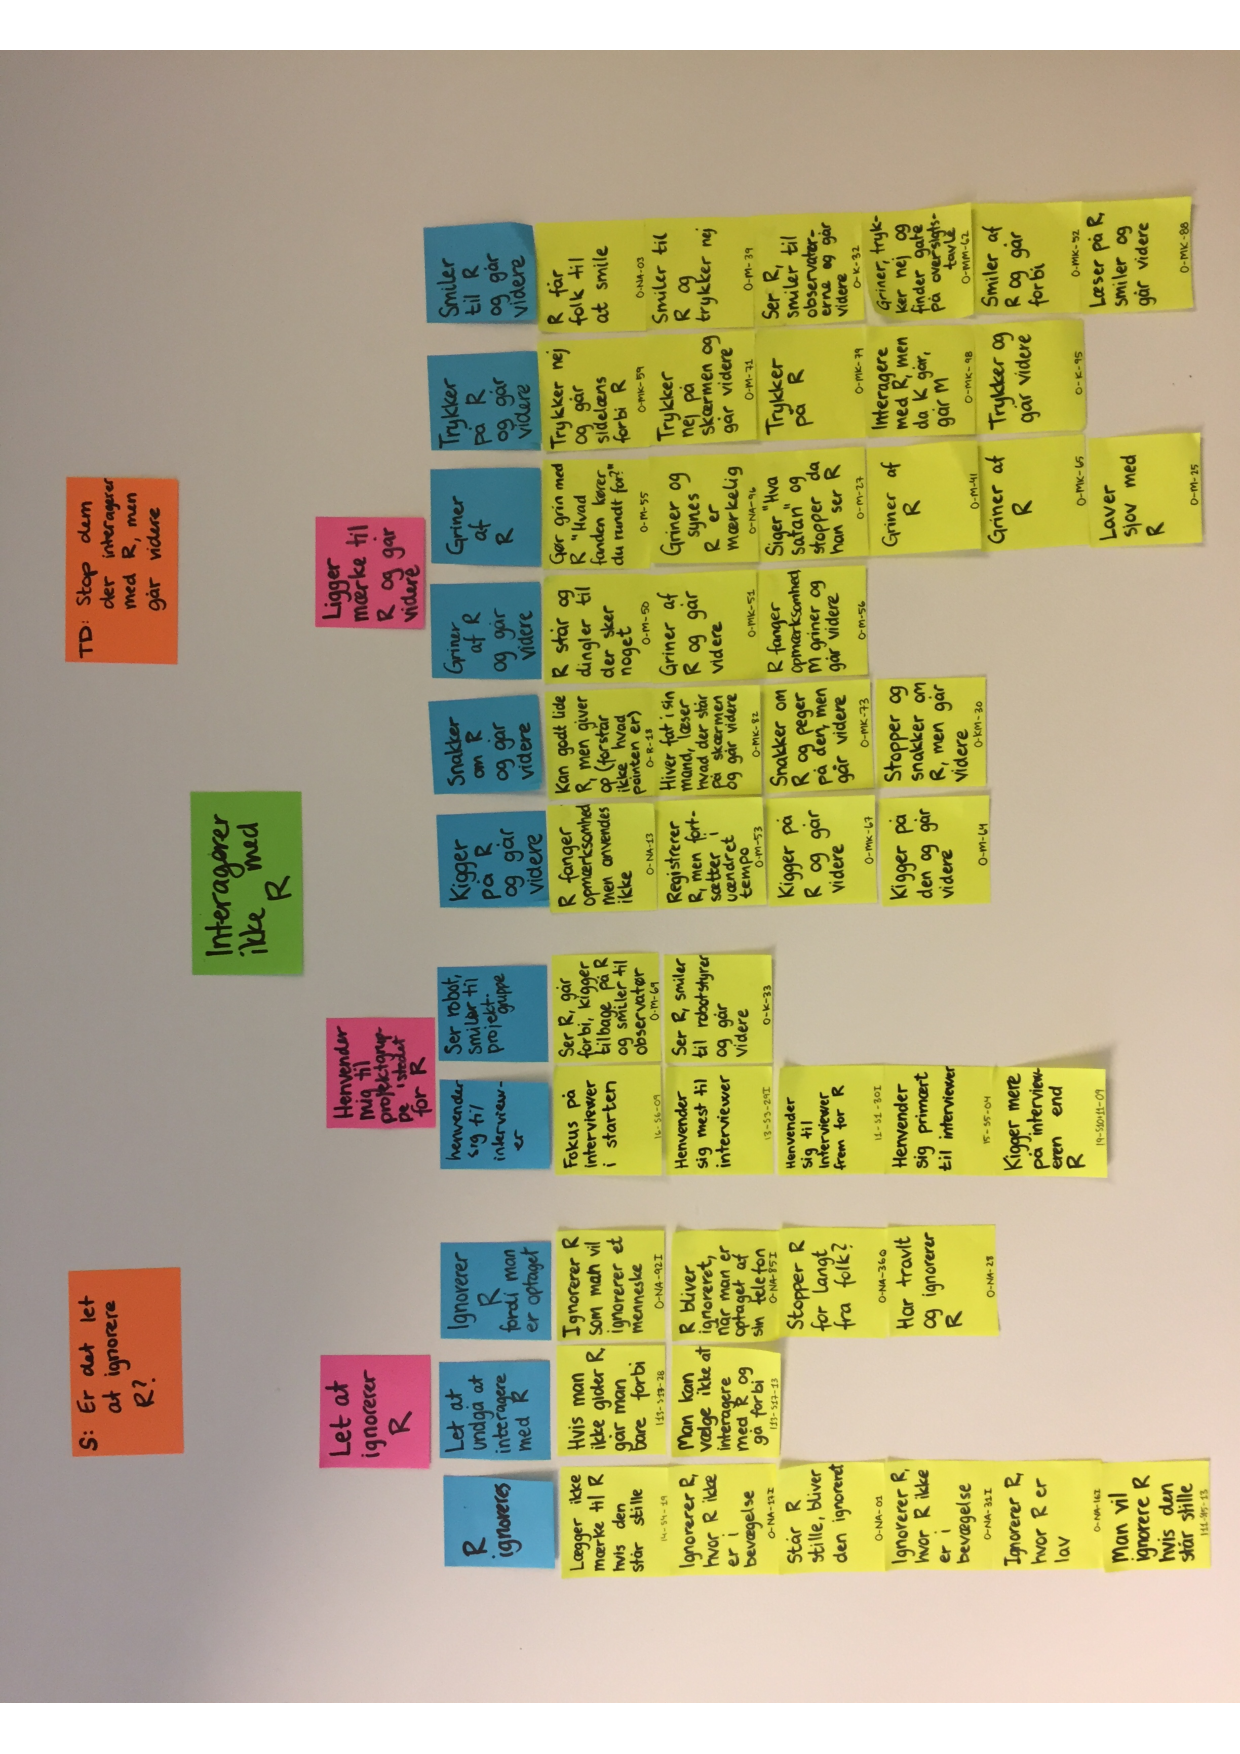
\includegraphics[width = 0.7\textwidth, angle = -90]{Figure/AffinityDiagram/InteragererIkkeMedR} 
\caption{Oversigt over den grønne kategori: \textit{Interagerer ikke med R}, hvor er \textit{R} angiver robot, med tilhørende \textit{affinity notes} placeret under henholdvist blå og pink labels, samt de udarbejde orange \textit{sticky notes}.}
\label{fig:AFInteragererIkkeMedR}
\end{figure}
\noindent
%
På \autoref{fig:AFInteragererIkkeMedR} fremgår to orange \textit{sticky notes}, hvoraf én er en idé til det næste testdesign, som relaterer sig til at de rejsende, der interagerer med robotten men ikke ender med at følge efter robotten stoppes og spørges ind til hvorfor de stoppede interaktionen. Da ordet \textit{ignorere} dækker over flere aspekter vælges det at omformulere udsagnet så det bedst muligt afspejler hvad der sigtes efter at måle, nemlig om det er muligt at undgå robotten, hvorfor udsagnet omformuleres til følgende potentielle skala spørgsmål:\blankline 
%
\begin{enumerate}
  \item Er det let at undgå R\blankline
\end{enumerate} 
\noindent
%
Til ovenstående potentielle skala spørgsmål kan følgende labels anvendes:
%
\begin{table}[H]
	\centering
	\begin{tabular}{l|c|c|c}
		SQ     & Venstre label & Midt punkt & Højre label \\\hline
		1   & Ekstremt svært & - & Ekstremt let                 
	\end{tabular}
\caption{Skala labels vedrørende hvor let det er at undgå robotten. \textit{SQ} er en forkortelse for skala spørgsmål.}
	\label{tab:IgnorerR} 
\end{table}
\noindent
%
Baseret på det potentielle skala spørgsmål samt tilhørende labels, der fremgår i \autoref{tab:IgnorerR}, vil det udgøre en unipolær skala uden et midt punkt. 
%
\newpage
\subsection{Skærmen virker ikke}
\label{ParametreSkaermenVirkerIkke}
%
\begin{figure}[H]
\centering
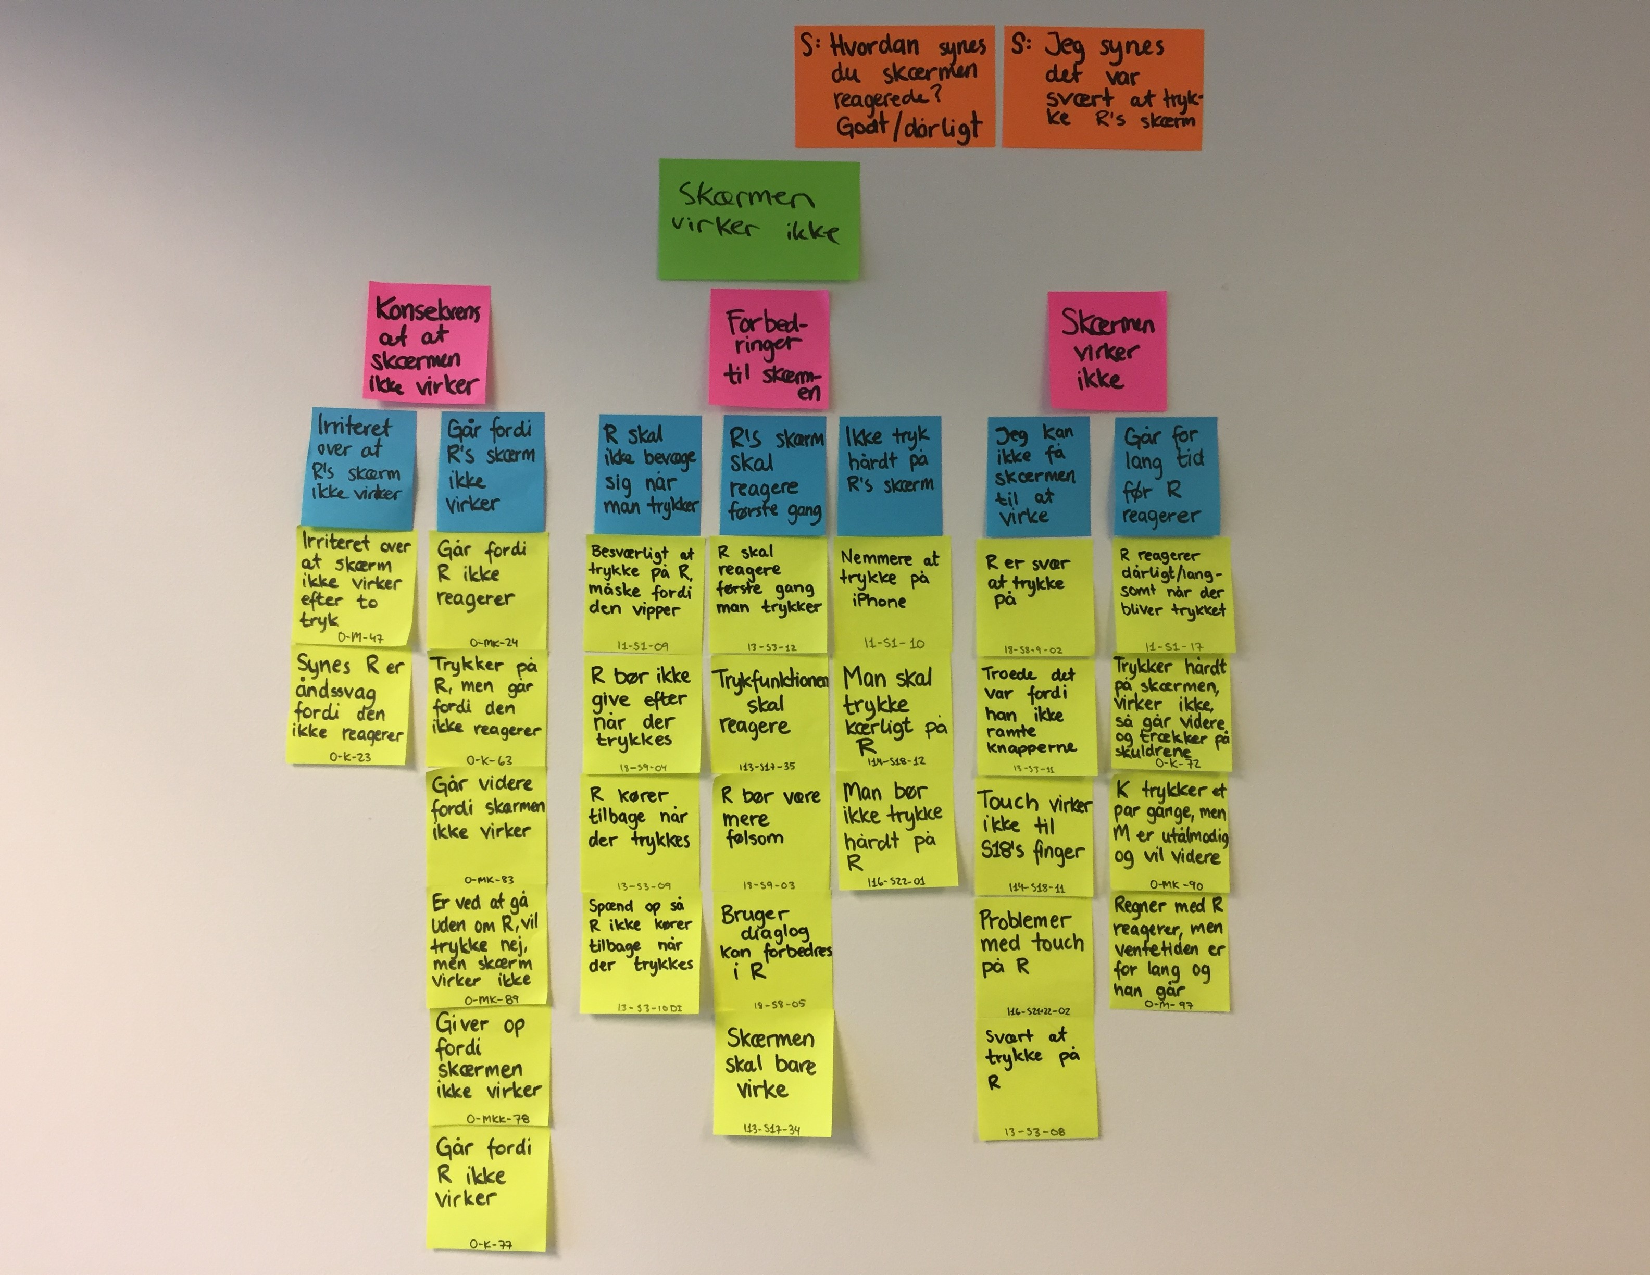
\includegraphics[width = 0.9\textwidth]{Figure/AffinityDiagram/SkaermenVirkerIkke} 
\caption{Oversigt over den grønne kategori: \textit{Skærmen virker ikke} med tilhørende \textit{affinity notes} placeret under henholdvist blå og pink labels, samt de udarbejde orange \textit{sticky notes}.}
\label{fig:AFSkaermVirkerIkke}
\end{figure}
\noindent
%
Da de to orange \textit{sticky notes} vedrører den samme problemstilling, at skærmen forvoldte problemer vælges det er sætte de to sammen og omformulere dem til følgende:\blankline
%
\begin{enumerate}
  \item Hvordan synes du skærmen virkede\blankline
\end{enumerate}
%
Til ovenstående potentielle skala spørgsmål kan følgende labels anvendes:
%
\begin{table}[H]
	\centering 
	\begin{tabular}{l|c|c|c}
		SQ     & Venstre label & Midt punkt & Højre label \\\hline
		1   & Ekstremt dårligt & Intet label & Ekstremt godt                 
	\end{tabular}
\caption{Skala labels vedrørende skærmen på robotten. \textit{SQ} er en forkortelse for skala spørgsmål.}
	\label{tab:SkaermenR}
\end{table}
\noindent
%
Det potentielle skala spørgsmål vil blive evalueret på en bipolær skala med et unavngivet midt punkt. Årsagen til at dette potentielle skala spørgsmål ikke ekskluderes, da det ikke er muligt for en designer at ændre på, er at det antages at hvordan skærmen virker har en indflydelse på hvordan testpersonerne evaluerer andre parametre. Derudover forventes det, at skærmen på den færdig udviklede robot ikke vil forårsage disse problemer, da brugergrænsefladen selvsagt ikke skal åbnes igennem \textit{Double}s applikation. 
\newpage
%
\subsection{R kan assistere mennesker}
\label{ParametreRKanAssistereMennesker}
%
\begin{figure}[H]
\centering
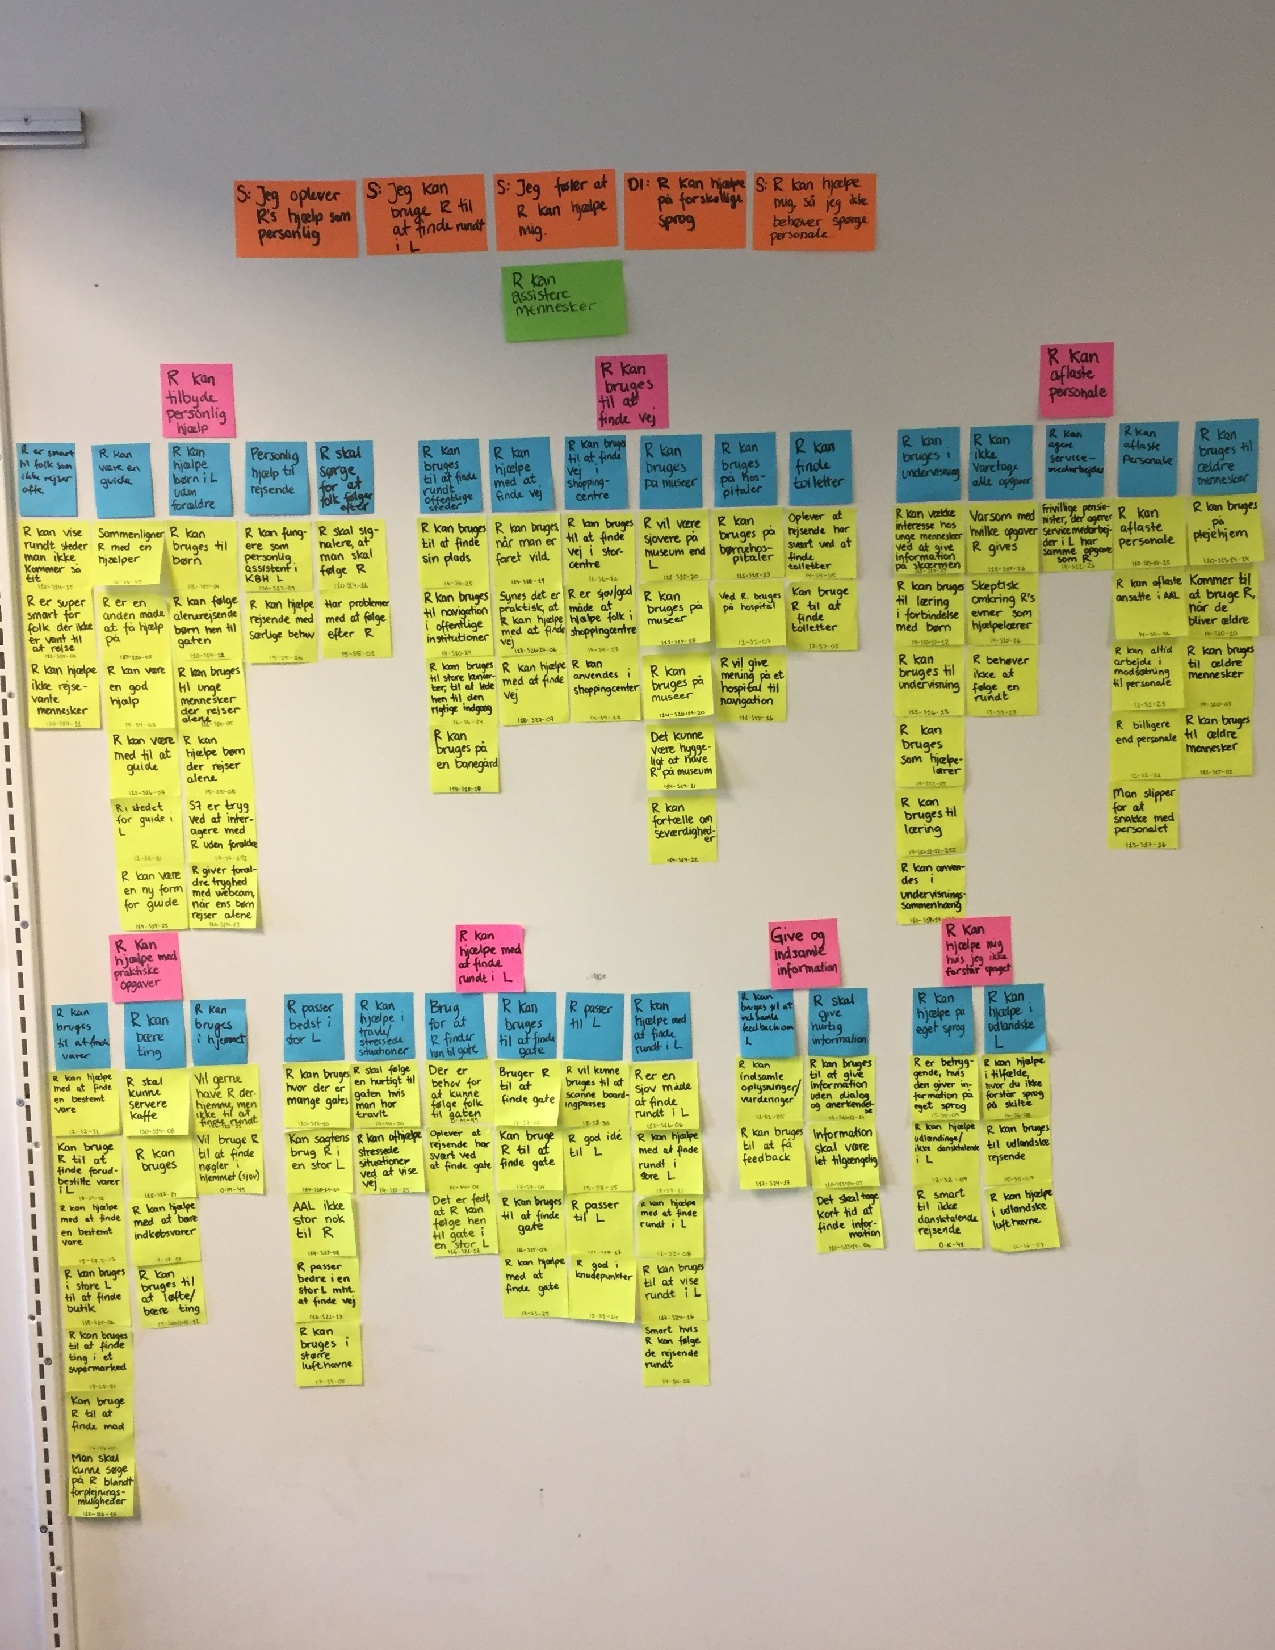
\includegraphics[width = 0.9\textwidth]{Figure/AffinityDiagram/RKanAssistereMennesker} 
\caption{Oversigt over den grønne kategori: \textit{R kan assistere mennesker}, hvor \textit{R} angiver robot og \textit{L} angiver lufthavn, med tilhørende \textit{affinity notes} placeret under henholdvist blå og pink labels, samt de udarbejde orange \textit{sticky notes}.}
\label{fig:AFRKanAssistereMennesker}
\end{figure}
\noindent
%
Baseret på de fire potentielle skala spørgsmål vælges det at sammensætte: \textit{Jeg kan bruge R til at finde rundt i L} med \textit{Jeg føler at R kan hjælpe mig} til et samlet potentielt skala spørgsmål, som fremgår i nedenstående. Derudover er fremgår der en design idé på \autoref{fig:AFRKanAssistereMennesker}, som vedrører at robotten bør kunne hjælpe på forskellige sprog og ikke kun på dansk.\blankline 
%
\begin{enumerate}
  \item Jeg oplever R's hjælp som personlig
  \item Jeg føler at R kan hjælpe mig
  \item R kan hjælpe mig så jeg ikke behøver at spørge personale\blankline
\end{enumerate}
\noindent
%
Til hver af de tre ovenstående potentielle skala spørgsmål kan følgende labels anvendes:
%
\begin{table}[H]
	\centering
	\begin{tabular}{l|c|c|c}
		SQ     & Venstre label & Midt punkt & Højre label \\\hline
		1   & Slet ikke personlig & - & Ekstremt personlig          \\\hline
		2   & Helt uenig & Intet label & Helt enig   \\\hline
		3   & Helt uenig & Neutral & Helt enig  
	\end{tabular}
\caption{Skala labels vedrørende hvorvidt robotten kan assistere mennesker. \textit{SQ} er en forkortelse for skala spørgsmål.}
	\label{tab:AssistererMennesker}
\end{table}
\noindent
%
Skalaen vedrørende hvorvidt robottens hjælp opleves som værende personlig vil blive evalueret på en unipolær skala. Hvor de to andre potentielle skala spørgsmål begge vil blive evalueret på en bipolær skala med et midt punkt henholdvist unavngivet og angivet med \textit{Neutral}.
\newpage
%
\subsection{R's væremåde}
\label{ParametreRsVaeremaade}
%
\begin{figure}[H]
\centering
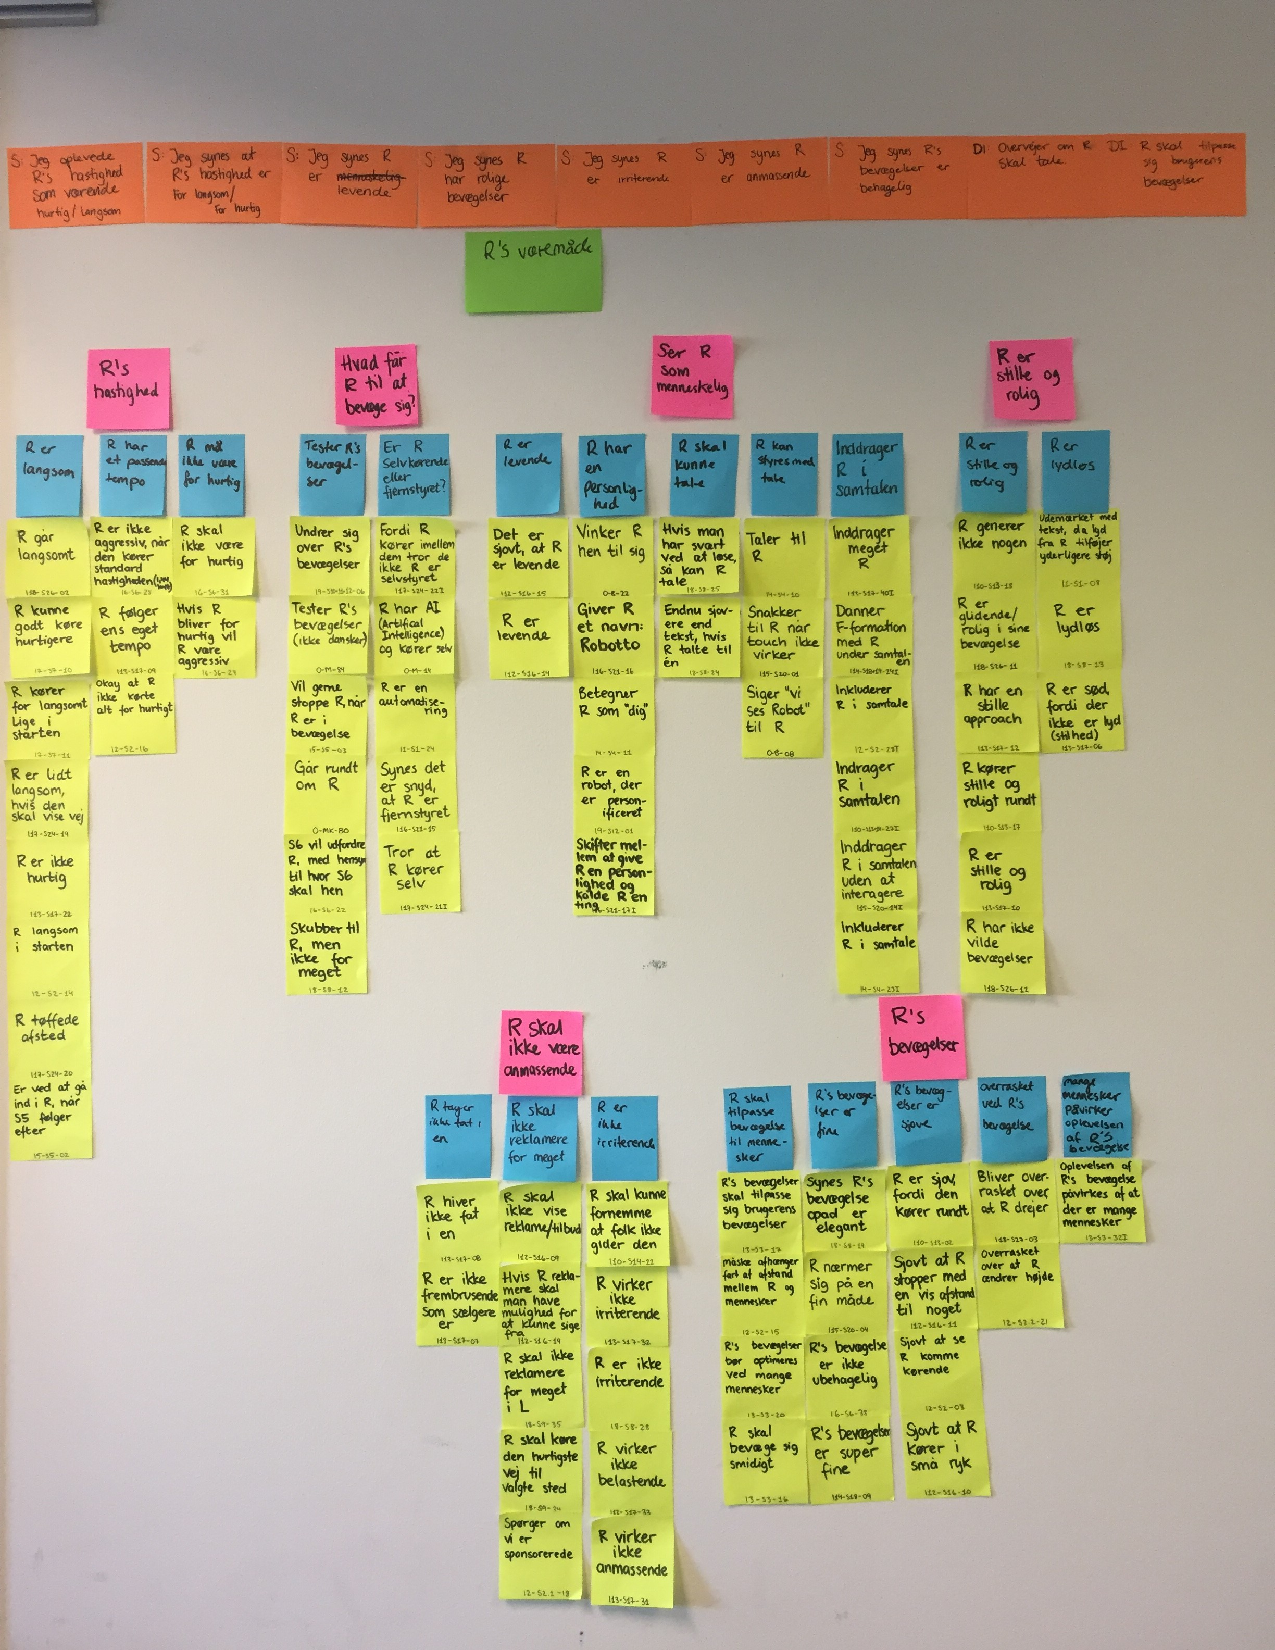
\includegraphics[width = 0.9\textwidth]{Figure/AffinityDiagram/RsVaeremaade} 
\caption{Oversigt over den grønne kategori: \textit{R's væresmåde}, hvor \textit{R} angiver robot, med tilhørende \textit{affinity notes} placeret under henholdvist blå og pink labels, samt de udarbejde orange \textit{sticky notes}.}
\label{fig:AFRsVaeremaade}
\end{figure}
\noindent
%
Ud af de ni orange \textit{sticky notes} er to design idéer hvor én relatere sig til at det bør overvejes om robotten skal tale og den anden relatere sig til at robotten skal tilpasse sine bevægelser afhængigt af brugerens bevægelser. Derudover er det valgt at sammensætte \textit{Jeg synes R's bevægelser er behagelige} med \textit{Jeg synes R har rolige bevægelser} til ét potentielt skala spørgsmål, listet som det første i nedenstående. Ydermere er det valgt at sammensætte \textit{Jeg oplevede R's hastighed som værende hurtig/langsom} med \textit{Jeg synes at R's hastighed er for langsom/for hurtig} til ét potentiel skala spørgsmål der vedrører robottens hastighed, listet som nummer to i nedenstående. De tre resterende bibeholdes: \blankline 
%
\begin{enumerate}
  \item Jeg synes at R's bevægelser er... 
  \item Jeg synes at R's hastighed er... 
  \item Jeg synes at R er irriterende
  \item Jeg synes at R er levende
  \item Jeg synes at R er anmassende\blankline
\end{enumerate}
%
Til hver af de fem ovenstående potentielle skala spørgsmål kan følgende labels anvendes:
%
\begin{table}[H]
	\centering 
	\begin{tabular}{l|c|c|c}
		SQ     & Venstre label & Midt punkt & Højre label \\\hline
		1   & Alt for rolige & Intet label & Alt for vilde     \\\hline
		2   & Alt for langsom & Fin & Alt for hurtig   \\\hline
		3   & Slet ikke irriterende & - & Ekstremt irriterende \\\hline
	 	4   & Slet ikke levende & - & Ekstremt levende         \\\hline
		5   & Slet ikke anmassende & - & Ekstremt anmassende             
	\end{tabular}
	\caption{Skala labels vedrørende robottens væremåde. \textit{SQ} er en forkortelse for skala spørgsmål.}
	\label{tab:VaeremaadeSkala}
\end{table}
\noindent
%
De to første potentielle skala spørgsmål vil begge blive evalueret på en bipolær skala med et midt punkt henholdvist uden et label og med label: \textit{Fin}. De tre resterende vil hver blive evalueret på en unipolær skala.
%
\subsection{Henvendelse}
\label{ParametreHenvendelse}
%
\begin{figure}[H]
\centering

\includegraphics[width = 0.9\textwidth]{Figure/AffinityDiagram/Henvendelse} 
\caption{Oversigt over den grønne kategori: \textit{Henvendelse} med tilhørende \textit{affinity notes} placeret under henholdvist blå og pink labels, samt de udarbejde orange \textit{sticky notes}.}
\label{fig:AFHenvendelse}
\end{figure}
\noindent
%
To ud af de syv orange \textit{sticky notes} er angivet som design idéer vedrørende robottens position relativt til brugeren, hvor robotten fortrinvist skal vende fronten mod brugeren samt være tæt på personen. Det vælges at ekskludere \textit{Jeg foretrækker at R/jeg henvender sig}, da det ikke er en parameter, der for en designer er mulig at ændre på. Derudover vælges det at omformulere \textit{Jeg synes R kom for tæt på} til \textit{Jeg synes R er intimiderende}. Denne omformulering er baseret på dels de blå labels samt \textit{affinity notes} kategoriseret under den pink label: \textit{R skal respektere intimsfæren}. Dette medføre at følgende potentielle skala spørgsmål formuleres: \blankline
%
\begin{enumerate}
  \item Jeg synes at R er imødekommende
  \item Jeg synes at R kom for tæt på
  \item Jeg synes at R stod i vejen
  \item Jeg blev overrasket over R's henvendelse 
  \item Jeg synes at R er intimiderende\blankline
\end{enumerate}
%
Til hver af de fem ovenstående potentielle skala spørgsmål kan følgende labels anvendes:
%
\begin{table}[H]
	\centering
	\begin{tabular}{l|c|c|c}
		SQ     & Venstre label & Midt punkt & Højre label \\\hline
		1   & Ekstremt afvisende & Intet label & Ekstremt imødekommende         \\\hline
		2   & Alt for tæt på & Intet label & Alt for langt fra   \\\hline
		3   & Slet ikke i vejen & -  & Ekstremt i vejen  \\\hline
	 	4   & Slet ikke overrasket &  -  & Ekstremt overrasket \\\hline
		5   & Slet ikke intimiderende & - & Ekstremt intimiderende           
	\end{tabular}
	\caption{Skala labels vedrørende robottens henvendelse. \textit{SQ} er en forkortelse for skala spørgsmål.}
	\label{tab:HenvendelseSkala} 
\end{table}
\noindent
%
Baseret på \autoref{tab:HenvendelseSkala} vil de to første potentielle skala spørgsmål blive evalueret på en bipolær skala med et midt punk som henholdvist er unavngivet og navngivet med \textit{Tilpas}. De tre resterende potentielle skala spørgsmål vil hver blive evalueret på en unipolær skala.
\newpage
%
\subsection{R's udseende}
\label{ParametreRsUdseende}
%
\begin{figure}[H]
\centering
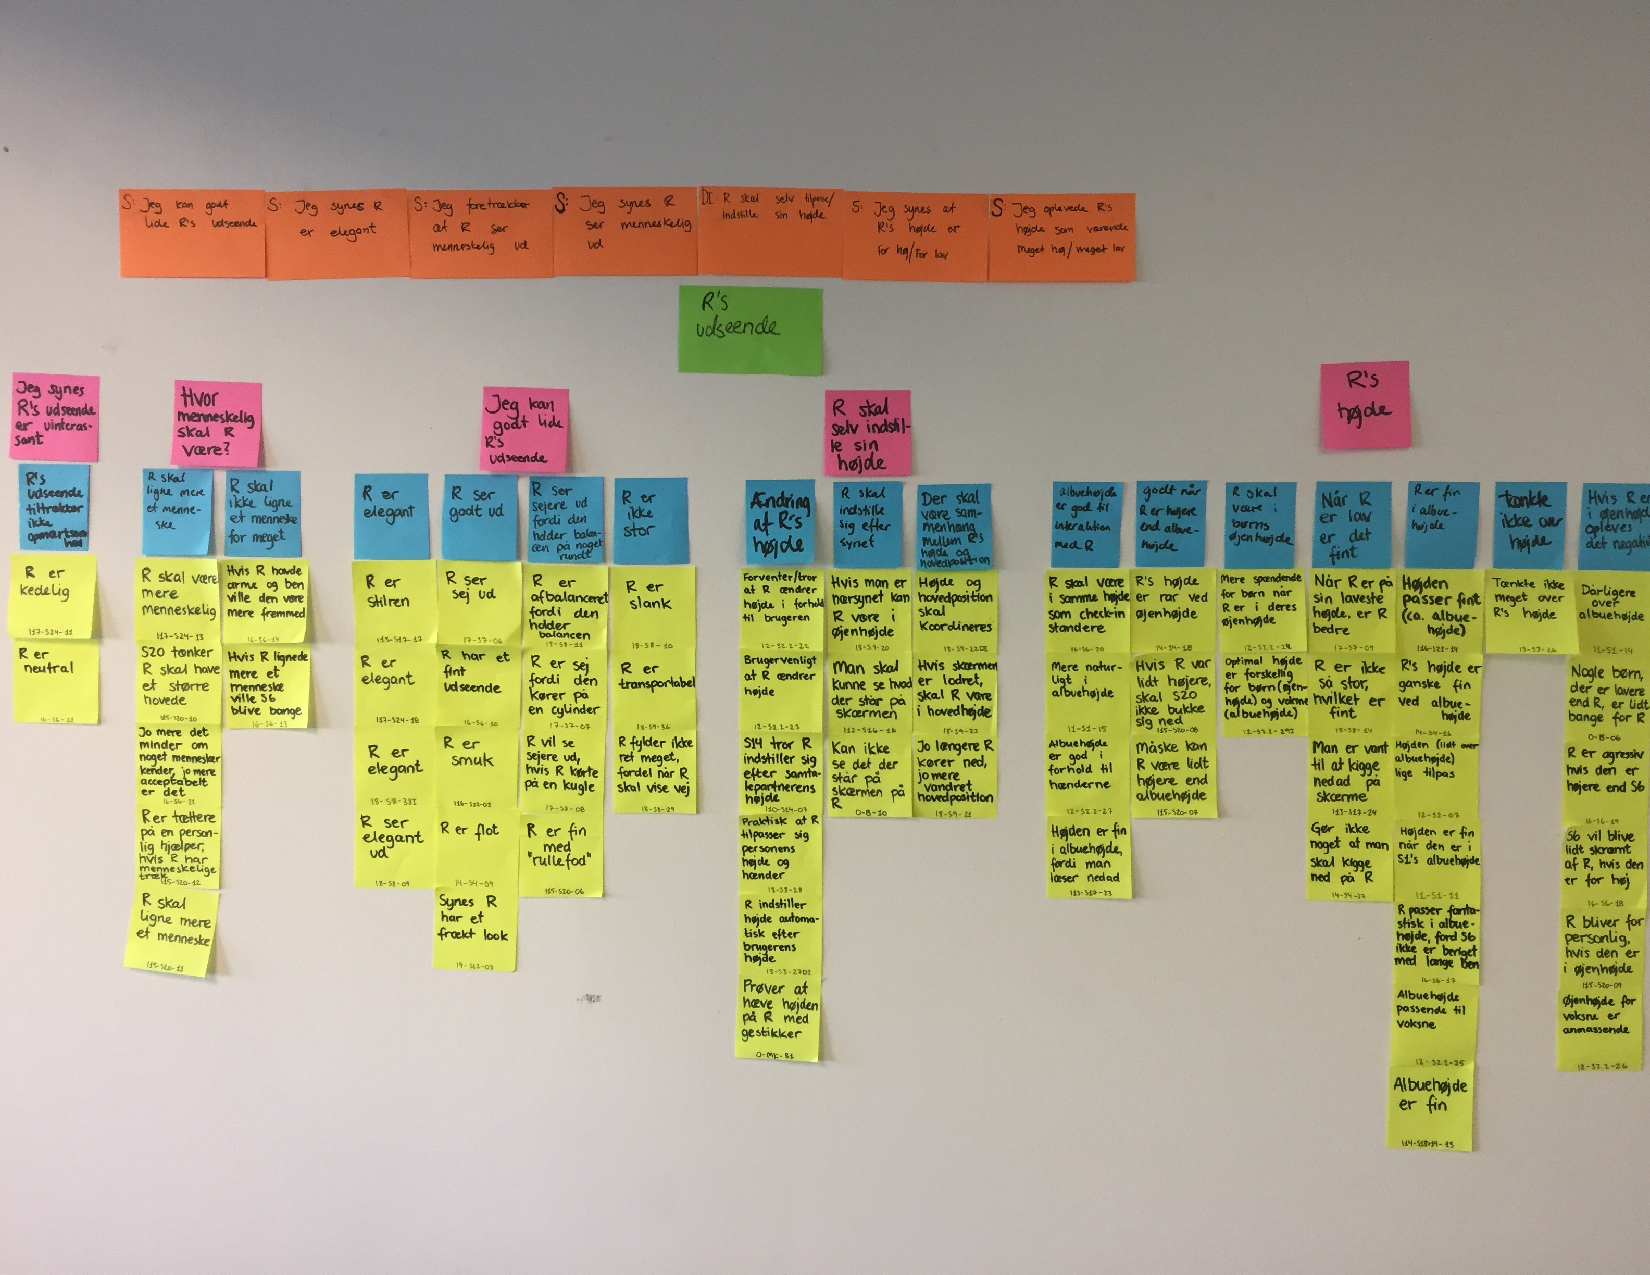
\includegraphics[width = 0.9\textwidth]{Figure/AffinityDiagram/RsUdseende} 
\caption{Oversigt over den grønne kategori: \textit{R's udseende}, hvor \textit{R} angiver robot, med tilhørende \textit{affinity notes} placeret under henholdvist blå og pink labels, samt de udarbejde orange \textit{sticky notes}.}
\label{fig:AFRsUdseende}
\end{figure}
\noindent
%
På \autoref{fig:AFRsUdseende} fremgår der én design idé, som vedrører at robotten automatisk skal indstille sin højde afhængigt af brugerens højde. Det vælges at sammensætte \textit{Jeg oplevede R's højde som værende meget høj/meget lav} med \textit{Jeg synes at R's højde er for høj/for lav} til et enkelt potentielt skala spørgsmål vedrørende robottens højde. Da det ikke er muligt for en designer at påvirke hvad en potentiel bruger foretrækker vælges det at sammensætte \textit{Jeg foretrækker at R ser menneskelig ud} med \textit{Jeg synes at R ser menneskelig ud}. De potentielle skala spørgsmål er som følger: \blankline
% 
\begin{enumerate}
  \item Jeg synes at R's højde er... 
  \item Jeg synes at R er elegant
  \item Jeg synes at R ser menneskelig ud
  \item Jeg kan godt lide R's udseende\blankline
\end{enumerate}
\newpage
%
Til hver af de fire ovenstående potentielle skala spørgsmål kan følgende labels anvendes:
%
\begin{table}[H]
	\centering
	\begin{tabular}{l|c|c|c}
		SQ     & Venstre & Midt punkt & Højre label \\\hline
		1   & Alt for lav  & Fin & Alt for høj        \\\hline
		2   & Slet ikke elegant & - & Ekstremt elegant         \\\hline
		3   & Slet ikke menneskelig & - & Ekstremt menneskelig         \\\hline
	 	4   & Helt uenig & - & Helt enig                   
	\end{tabular}  
	\caption{Skala labels vedrørende robottens udseende. \textit{SQ} er en forkortelse for skala spørgsmål.}
	\label{tab:UdseendeSkala}       
\end{table}
\noindent
%
Baseret på \autoref{tab:UdseendeSkala} er det kun skalaen, som vedrører robottens højde, der evalueres på en bipolær skala med midt punktet \textit{Fin}. De resterende tre potentielle skala spørgsmål bliver alle evalueret på en unipolær skala. 
%
\subsection{Interesse for R}
\label{ParametreInteresseForR}
%
\begin{figure}[H]
\centering
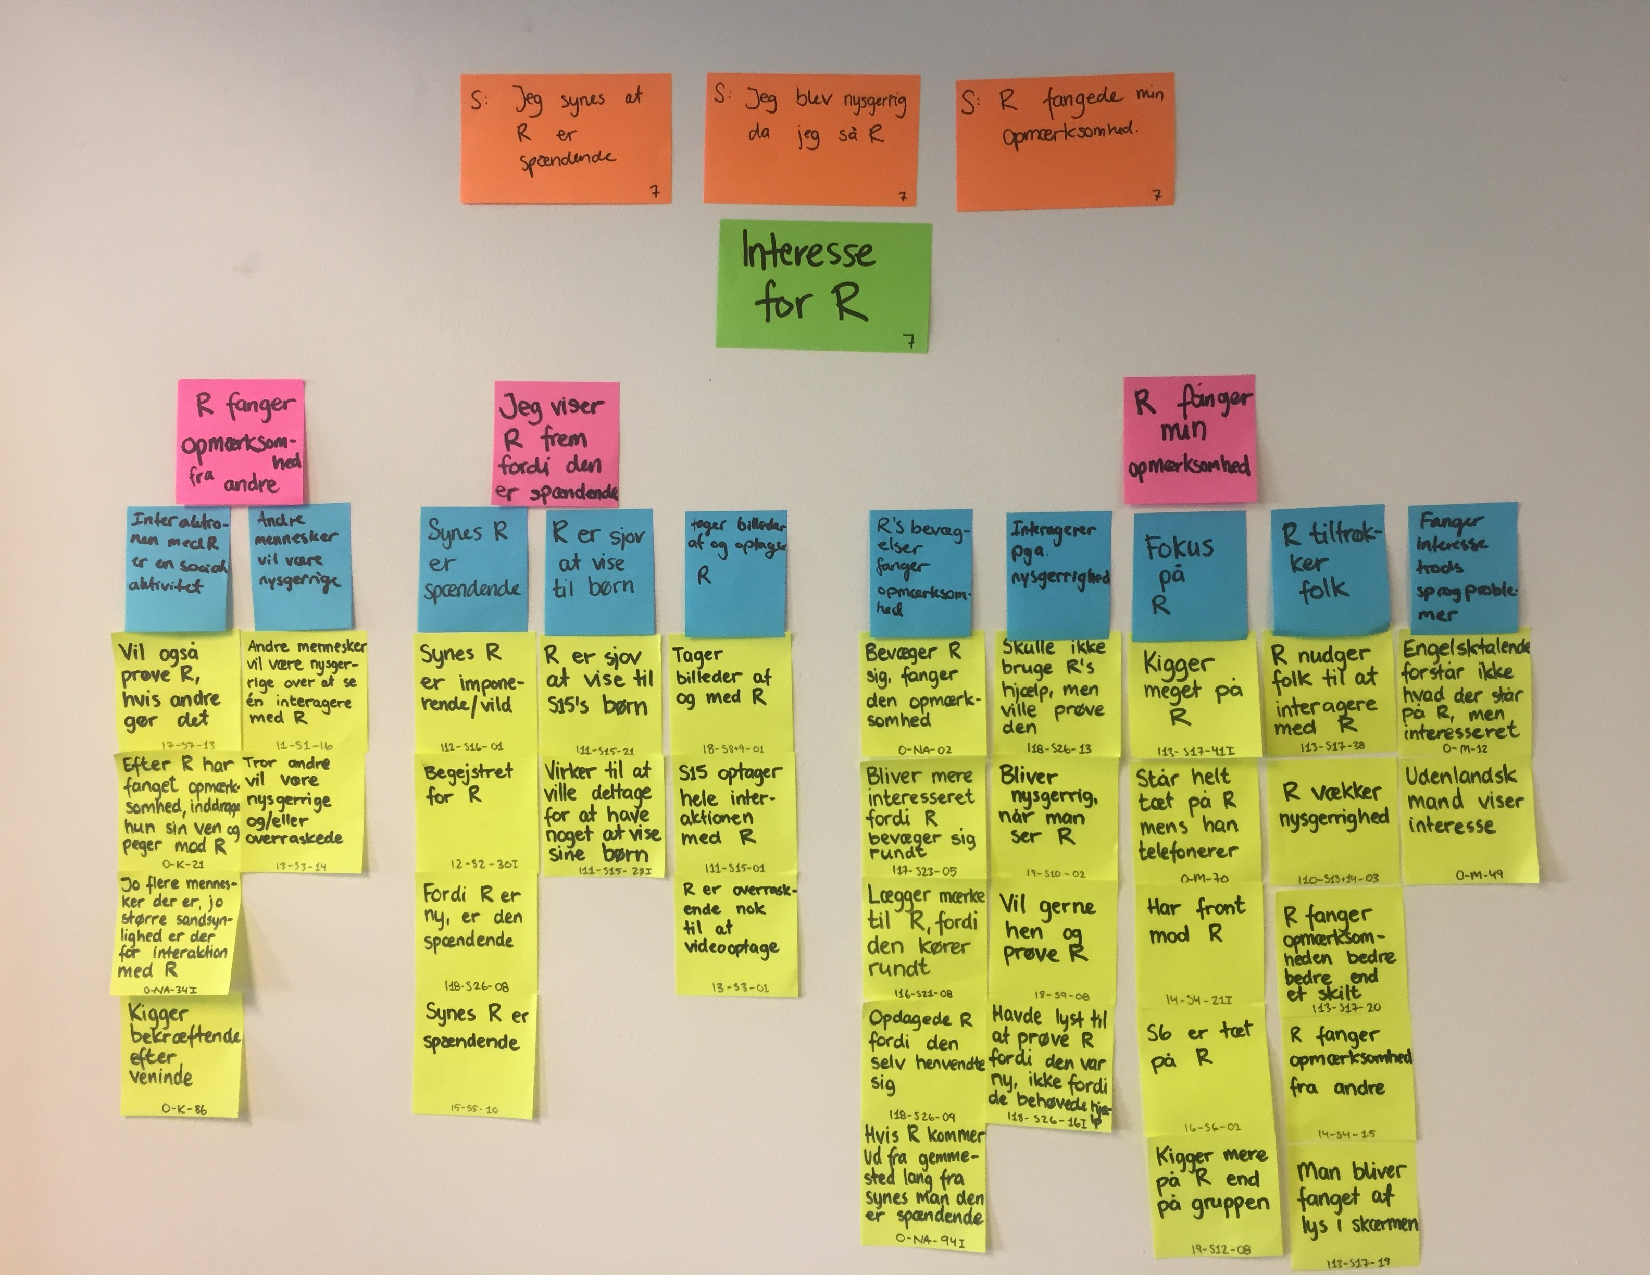
\includegraphics[width = 0.9\textwidth]{Figure/AffinityDiagram/InteresseForR} 
\caption{Oversigt over den grønne kategori: \textit{Interesse for R}, hvor \textit{R} angiver robot, med tilhørende \textit{affinity notes} placeret under henholdvist blå og pink labels, samt de udarbejde orange \textit{sticky notes}.}
\label{fig:AFInteresseForR}
\end{figure}
\noindent
%
Det vælges at sammensætte \textit{Jeg blev nysgerrig da jeg så R} med \textit{Jeg synes at R er spændende} til ét potentielt skala spørgsmål, da det antages at de vedrører det samme. De to potentielle skala spørgsmål er som følger: \blankline
%
\begin{enumerate}
  \item R fangede min opmærksomhed
  \item Jeg synes at R er spændende\blankline
\end{enumerate}
%
Til hver af de to ovenstående potentielle skala spørgsmål kan følgende labels anvendes:
%
\begin{table}[H]
	\centering 
	\begin{tabular}{l|c|c|c}
		SQ     & Venstre label & Midt punkt & Højre label \\\hline
		1   & Slet ikke & - & Ekstremt meget          \\\hline
		2   & Slet ikke spændende & - & Ekstremt spændende                 
	\end{tabular}
\caption{Skala labels vedrørende interesse for robotten. \textit{SQ} er en forkortelse for skala spørgsmål.}
	\label{tab:InteresseForR}
\end{table}
\noindent
%
Baseret på ovenstående \autoref{tab:InteresseForR} vil de to potentielle skala spørgsmål begge blive evalueret på en unipolær skala. 
%
\subsection{Positiv overfor R}
\label{ParametrePositivOverforR}
%
\begin{figure}[H]
\centering
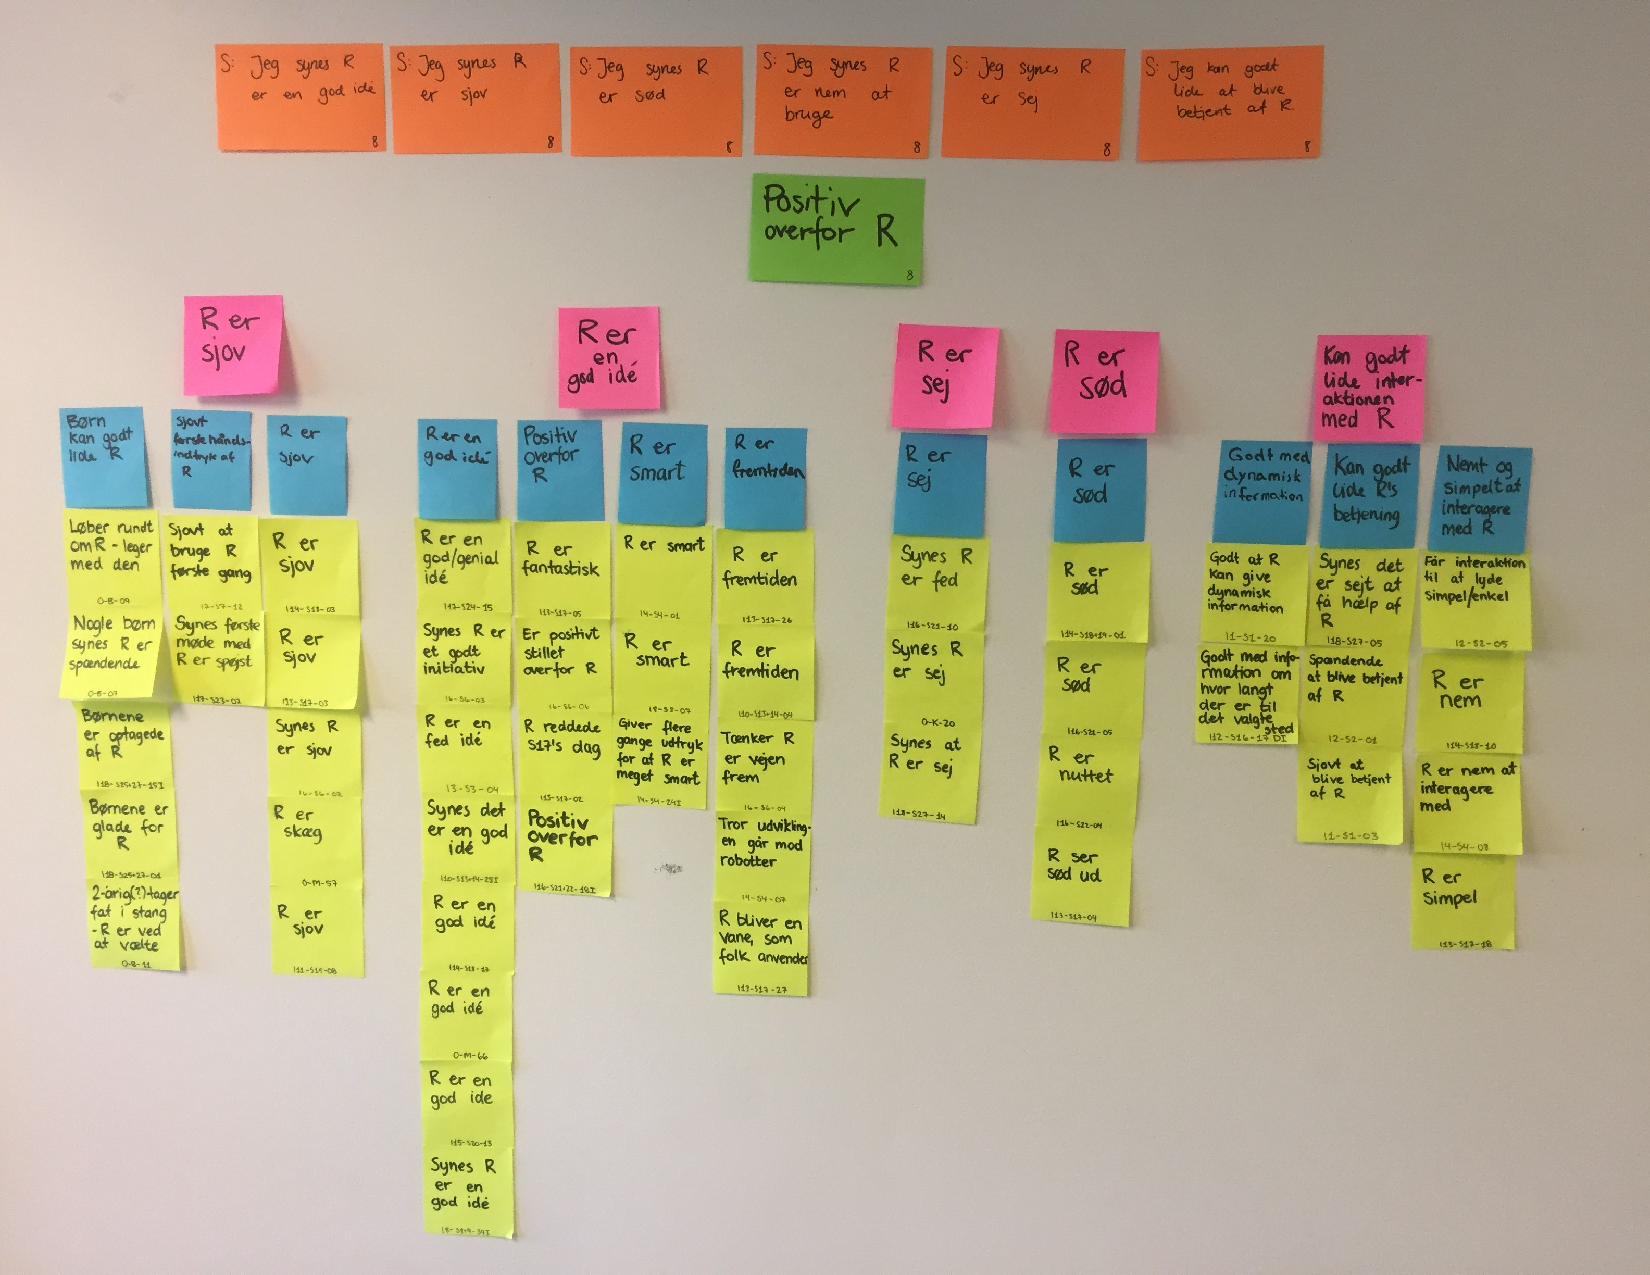
\includegraphics[width = 0.9\textwidth]{Figure/AffinityDiagram/PositivOverforR} 
\caption{Oversigt over den grønne kategori: \textit{Positiv overfor R}, hvor \textit{R} angiver robot, med tilhørende \textit{affinity notes} placeret under henholdvist blå og pink labels, samt de udarbejde orange \textit{sticky notes}.}
\label{fig:AFPositivOverforR}
\end{figure}
\noindent
%
Det vælges at ekskludere \textit{Jeg synes R er en god idé}, da det ikke er muligt for en designer at ændre på hvorvidt potentielle brugere betragter robotten som værende en god idé. Derudover vælges det at sammensætte \textit{Jeg synes R er nem at bruge} med {Jeg har brug for hjælp til at bruge R} fra den grønne kategori: \textit{Kendskab til teknologi}, da det vurderes at de to udtryk er modsætninger, som beskriver den samme oplevelse, hvorfor skala spørgsmålet vil fremgå af \fullref{ParametreKendskabTilTeknologi}.\blankline  
%
\begin{enumerate}
  \item Jeg synes at R er sød
  \item Jeg synes at R er sjov
  \item Jeg synes at R er sej
  \item Jeg kan godt lide at blive betjent af R\blankline
\end{enumerate}
%
Til hver af de fire ovenstående potentielle skala spørgsmål kan følgende labels anvendes:
%
\begin{table}[H]
	\centering
	\begin{tabular}{l|c|c|c}
		SQ     & Venstre label & Midt punkt & Højre label \\\hline
		1   & Slet ikke sød & - & Ekstremt sød      \\\hline
		2   & Slet ikke sjov & - & Ekstremt sjov \\\hline
		3   & Slet ikke sej & - & Ekstremt sej \\\hline
		4   & Slet ikke & - & Ekstremt meget
	\end{tabular}
\caption{Skala labels vedrørende ens positive indstilling i henhold til robotten. \textit{SQ} er en forkortelse for skala spørgsmål.}
\label{tab:PositivR} 
\end{table}
\noindent
%
Baseret på ovenstående \autoref{tab:PositivR} vil alle fire potentielle skala spørgsmål blive evalueret på en unipolær skala. 
%
\subsection{Kendskab til teknologi}
\label{ParametreKendskabTilTeknologi}
%
\begin{figure}[H]
\centering
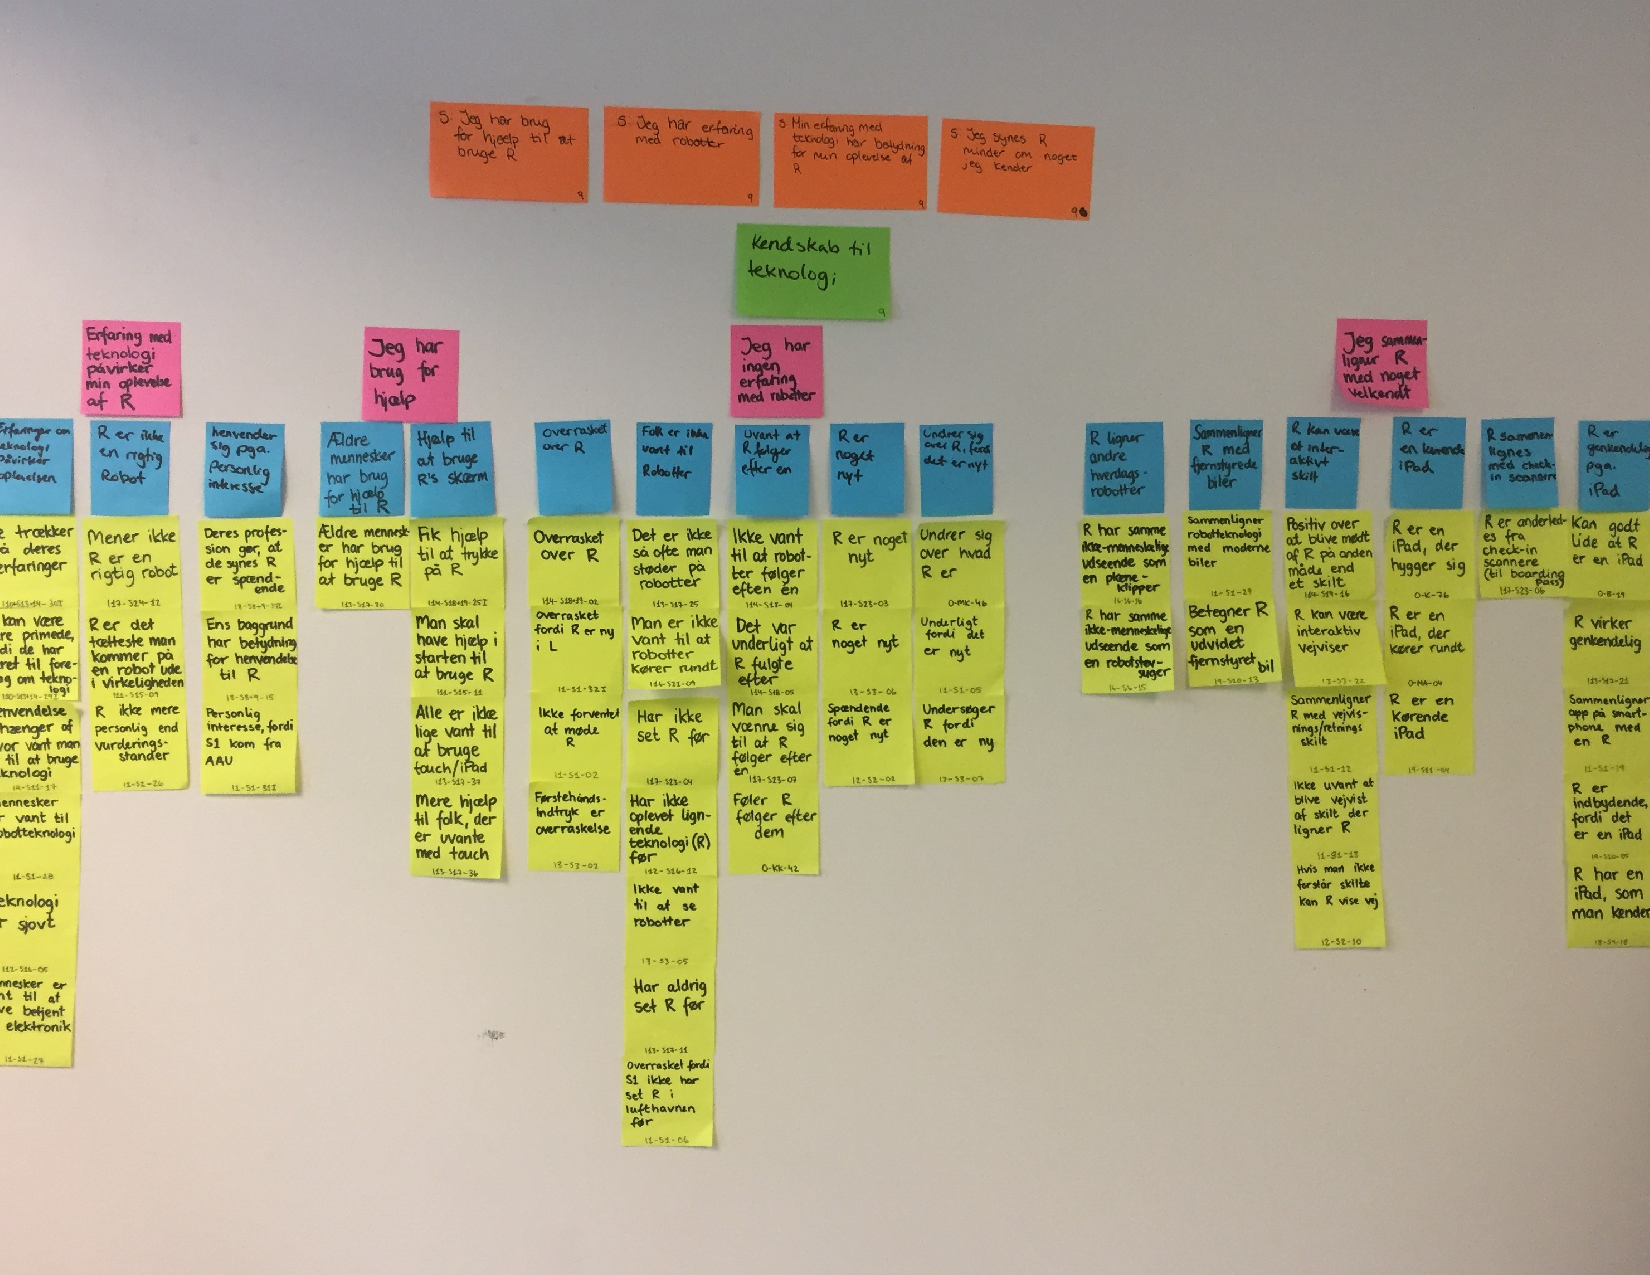
\includegraphics[width = 0.9\textwidth]{Figure/AffinityDiagram/KendskabTilTeknologi} 
\caption{Oversigt over den grønne kategori: \textit{Kendskab til teknologi} med tilhørende \textit{affinity notes} placeret under henholdvist blå og pink labels, samt de udarbejde orange \textit{sticky notes}.}
\label{fig:AFKendskabTilTeknologi}
\end{figure}
\noindent
%
Som nævnt sammensættes \textit{Jeg synes R er nem at bruge} fra \autoref{ParametrePositivOverforR} med \textit{Jeg har brug for hjælp til at bruge R} til ét enkelt potentielt skala spørgsmål, som vedrører hvordan det var at bruge robotten. De resterende tre udsagn: \textit{Jeg har erfaring med robotter}, \textit{Min erfaring med teknologi har betydning for min oplevelse af R} samt \textit{Jeg synes R minder om noget jeg kender} sammensættes. Det skyldes hovedsageligt at de to førstnævnte udsagn ikke er noget en designer har mulig for at ændre og selvom det potentielt er muligt at designe robotten, som noget velkendt er det ikke muligt at vide hvad potentielle brugere da sammenligner robotten med. Det vurderes dog, at brugerens kendskab til teknologier og robotter kan have indflydelse på hvordan andre parametre evalueres, hvorfor det vælges at formulere dette som et skala spørgsmål. Dette skala spørgsmål vil ikke indgå på samme måde som de resterende, men vil indgå som en del af at indsamle demografisk information fra testpersonerne. De to potentielle skala spørgsmål er formuleret som følger:\blankline
%
\begin{enumerate}
  \item Hvordan var det at bruge R
  \item Hvor meget kendskab har du til teknologi/robotter\blankline 
\end{enumerate}
%
Til hver af de to ovenstående potentielle skala spørgsmål kan følgende labels anvendes:
%
\begin{table}[H]
	\centering 
	\begin{tabular}{l|c|c|c}
		SQ     & Venstre label & Midt punkt & Højre label \\\hline
		1   & Ekstremt svært & Intet label & Ekstremt nemt          \\\hline
		2   & Slet ingen kendskab & - & Ekstremt meget kendskab 
	\end{tabular}
\caption{Skala labels vedrørende kendskab til teknologi. \textit{SQ} er en forkortelse for skala spørgsmål.}
	\label{tab:KendskabTilTek}
\end{table}
\noindent
%
Baseret på \autoref{tab:KendskabTilTek} vil det første potentielle skala spørgsmål relateret til hvordan den var at bruge robotten, blive evalueret på en bipolær skala med unavngivet midt punkt. Det andet potentielle skala spørgsmål, som vil indgå i indsamlingen af demografisk data, vil blive evalueret på en unipolær skala. 
\newpage
%
\subsection*{Tillid til R}
%
\begin{figure}[H]
\centering
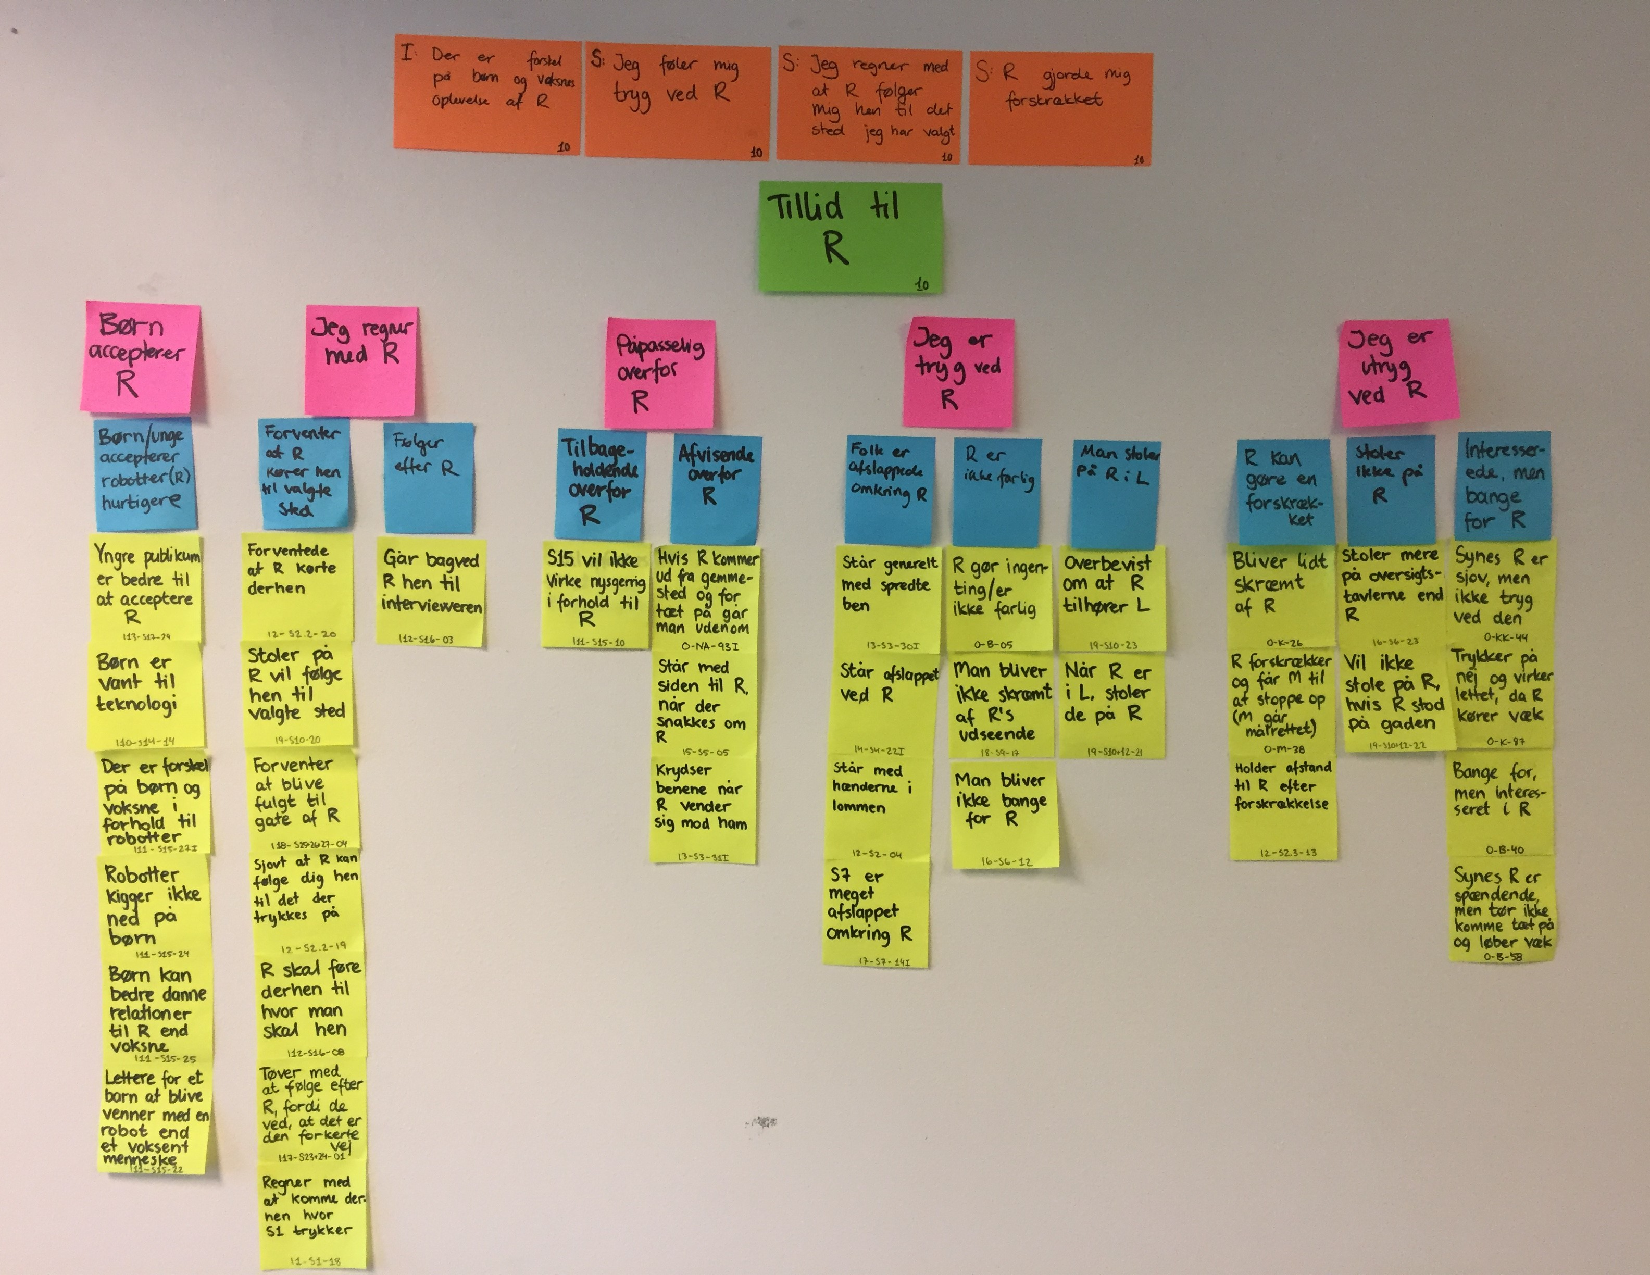
\includegraphics[width = 0.9\textwidth]{Figure/AffinityDiagram/TillidTilR} 
\caption{Oversigt over den grønne kategori: \textit{Tillid til R}, hvor \textit{R} angiver robot, med tilhørende \textit{affinity notes} placeret under henholdvist blå og pink labels, samt de udarbejde orange \textit{sticky notes}.}
\label{fig:AFTillidTilR}
\end{figure}
\noindent
%
På \autoref{fig:AFTillidTilR} fremgår der en orange \textit{sticky note} noteret med et \textit{I} efterfulgt af et udsagn. \textit{I} står for indsigt, hvor det i dette tilfælde vedrører at der er forskel på hvordan børn og voksne oplever interaktionen med robotten. Det er derfor hverken noget en designer vil kunne ændre på eller noget der skal være en del af det næste testdesign. De resterende tre orange \textit{sticky notes} er dog formuleret som potentielle skala spørgsmål: \blankline
%
\begin{enumerate}
  \item Jeg føler mig tryg ved R
  \item Jeg regner med at R følger mig hen til det sted jeg har valgt
  \item R gjorde mig forskrækket\blankline
\end{enumerate}
%
Til hver af de to ovenstående potentielle skala spørgsmål kan følgende labels anvendes:
%
\begin{table}[H]
	\centering 
	\begin{tabular}{l|c|c|c}
		SQ  & Venstre label & Midt punkt & Højre label \\\hline
		1   & Ekstremt utryg & Intet label & Ekstremt tryg  \\\hline
		2   & Helt uenig & Neutral & Helt enig \\ \hline
		3   & Slet ikke forskrækket & -  & Ekstremt forskrækket 
	\end{tabular} 
	\caption{Skala labels vedrørende tillid til robotten. \textit{SQ} er en forkortelse for skala spørgsmål.}
	\label{tab:TillidSkala}       
\end{table}
\noindent
%
De to første potentielle skala spørgsmål vil blive evalueret på en bipolær skala med midt punkt henholdvist unavngivet og navngivet med \textit{Neutral}, jævnfør \autoref{tab:TillidSkala}. Det sidste potentielle skala spørgsmål vil derimod blive evalueret på en unipolær skala. \blankline
%
Igennem de foregående afsnit har det været muligt at reducere antallet af udsagn fra 42 til 30 potentielle skala spørgsmål, hvoraf ét vil blive anvendt i forbindelse med indsamling af demografisk data. Dog vurderes det, at det er muligt med yderligere reducering af antallet af potentielle skala spørgsmål for at testpersonerne, som skal evaluere interaktionen med robotten ikke skal forhold sig til 30 skalaer. Derudover antages det at nogen af de potentielle skala spørgsmål reelt set måler det samme, hvorfor det er hensigtsmæssigt at sammensætte dem. I det følgende afsnit vil der derfor blive fokuseret på at udvælge og reducere antallet potentielle skala spørgsmål samt omformulerer spørgsmålene, hvis nødvendigt. 
